\section{Página da Comunidade OSC - Organizações da Sociedade Civil}
\label{Att:PaginaComunidade}

\begin{figure}[h]
\center
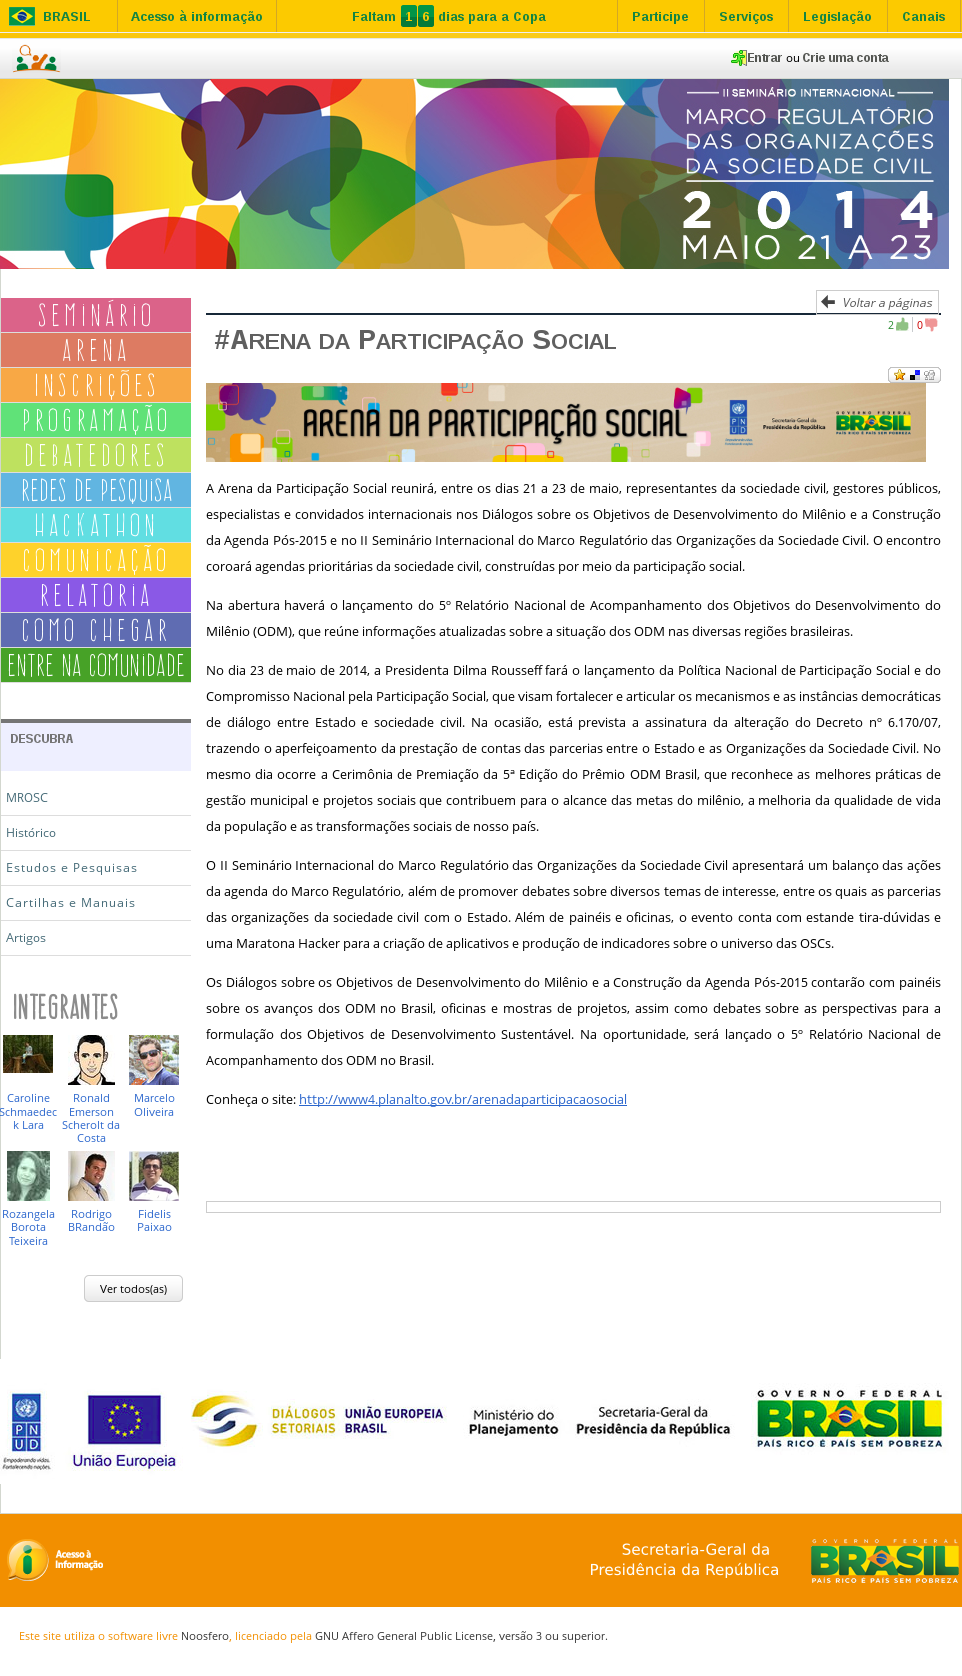
\includegraphics[scale=0.2]{tela-comunidade.png}
\caption{Página da comunidade OSC}
\label{fig:tela-comunidade}
\end{figure}

\newpage
\section{CSS do cabeçalho do tema de comunidade}
\label{Att:CabecalhoComunidade}

{\tiny
  \begin{verbatim}
    /* Header Effect */
    .header-content {
        height: 5px;
        transition-duration: 0.6s;
        overflow: hidden;
    }
    .header-content:hover,
    .header-content *:focus + .header-content,
    .header-content *:focus > .header-content {
        height: 173px;
    }
  \end{verbatim}
}

\section{Código javascript para incluir uma classe identificadora}
\label{Att:CodigoJsLinkColoridos}

{\tiny
  \begin{verbatim}
    jQuery('.link-list-block').first().wrap("<div class='colored-links'></div>");
  \end{verbatim}
}

\section{Código CSS para estilizar os blocos com o padrão colorido}
\label{Att:CodigoCSSLinkColoridos}

{\tiny
  \begin{verbatim}
    /* Colored links block */
    
    #content .colored-links .link-list-block li a,
    #content .colored-links .link-list-block li a.link-this-page,
    #box-organizer .colored-links .link-list-block li a,
    #box-organizer .colored-links .link-list-block li a.link-this-page {
      font-size: 28px;
      letter-spacing: 5px;
      background-color: transparent;
      color: #FFF;
      border-right: none;
    }
    
    #content .colored-links .link-list-block li:hover {
      opacity: 0.8;
      font-weight: bold;
      color: #FFF;
    }
    
    #content .colored-links .link-list-block li,
    #box-organizer .colored-links .link-list-block li {
      font-family: 'frente_h1regular';
      text-align: center;
      background-color: #db6389;
    }
    
    #content .colored-links .link-list-block li + li {
      background-color: #dd7b62;
    }
    
    #content .colored-links .link-list-block li + li + li {
      background-color: #f8a845;
    }
    
    #content .colored-links .link-list-block li + li + li + li {
      background-color: #60e278;
    }
    
    #content .colored-links .link-list-block li + li + li + li + li {
      background-color: #bee15f;
    }
    
    #content .colored-links .link-list-block li + li + li + li + li + li {
      background-color: #61b5e1;
    }
    
    #content .colored-links .link-list-block li + li + li + li + li + li + li {
      background-color: #61dee2;
    }
    
    #content .colored-links .link-list-block li + li + li + li + li + li + li + li {
      background-color: #fed22b;
    }
    
    #content .colored-links .link-list-block li + li + li + li + li + li + li + li +
    li {
      background-color: #8a59e6;
    }
    
    #content .colored-links .link-list-block li + li + li + li + li + li + li + li +
    li + li {
      background-color: #5F6CB2;
    }
    
    #content .colored-links .link-list-block li + li + li + li + li + li + li + li +
    li + li + li {
      background-color: #47A227;
    }
    
    #content .colored-links .link-list-block li + li + li + li + li + li + li + li +
    li + li + li + li {
      background-color: #316620;
    }
    
    #content .colored-links .link-list-block li + li + li + li + li + li + li + li +
    li + li + li + li + li {
      background-color: #FBB959;
    }
    
    #content .colored-links .link-list-block li + li + li + li + li + li + li + li +
    li + li + li + li + li + li {
      background-color: #FCC72B;
    }
    
    #content .colored-links .link-list-block li a:hover {
      color: #FFF;
      font-weight: bold;
      background: inherit;
    }
  \end{verbatim}
}

\section{Código javascript para substituir o texto do menu quando o mouse passa
por sobre ele}
\label{Att:CodigoJsHoverLinks}

{\tiny
  \begin{verbatim}
    var $replaceOnHover = {
      'before': 'after',
      'Comunicação': 'colaborativa',
      'Experiência': 'colaborativa',
      'Relatoria': 'compartilhada',
      'Convidados': 'confirmados',
      'Arena': 'participação social',
      'Como Chegar': 'mais informações'
    }

    var $specialCases = {
      'case': 'change',
      'participação social': 'letter-spacing',
      'mais informações': 'letter-spacing',
      'Rede de pesquisa': 'letter-spacing',
      'Rede de Pesquisa': 'letter-spacing'
    }

    var before;
    var after;

    $('.link-list-block a').hover (
      function() {
        var element = $(this);
        before = element.html();
        after = $replaceOnHover[before];
        var changeSpecial = $specialCases[after];

        if (after) {
          element.html(after);
        }
        if (changeSpecial) {
          element.css(changeSpecial, '1px');
        }
      },
      function() {
        var element = $(this);
        if (after) {
          element.html(before).css('letter-spacing', '5px');
        }
      }
    );
  \end{verbatim}
}

\section{Menu de administração da comunidade}
\label{Att:MenuAdministracao}

{\tiny
  \begin{verbatim}
    <% if logged_in? && profile.admins.include?(user) %>
      <div id="admin-bts">
        <a id="cmm-admin" class="quick-admin-link" href='<%=
    "/myprofile/#{profile.identifier}" %>'>Admin OSC</a>
        <a id="edit-blocks" class="quick-admin-link" href='<%=
    "/myprofile/#{profile.identifier}/profile_design" %>'>Editar blocos</a>
        <a id="upload-image" class="quick-admin-link" href='<%=
    "/myprofile/#{profile.identifier}/cms/upload_files" %>'>Subir imagem</a>
        <a id="highlight-image" class="quick-admin-link" href='<%=
    "/myprofile/#{profile.identifier}/cms/view/71603" %>'>Imagem para
    destaque<br/>(755px &times; 276px)</a>
        <a id="new-post" class="quick-admin-link" href='<%=
    "/myprofile/#{profile.identifier}/cms/view/61118" %>'>Novo post</a>
      </div>
    <% end %>
  \end{verbatim}
}
